\documentclass[spanish,notes=hide]{beamer}

%Para crear una versión 'handout' (Copyright: Diego Berrueta)
%\documentclass[handout,notes=show]{beamer}

\usetheme{Warsaw}
\usepackage{beamerthemesplit}

\usepackage[spanish]{babel}
\usepackage[utf8]{inputenc}
\usepackage{listings}
\usepackage{graphicx}
\usepackage{colortbl}

\title{SWAML}
\subtitle{Publicaci\'on de listas de correo en Web Sem\'antica}
\author{Sergio Fern\'andez L\'opez}
\institute{%
	\href{http://swaml.berlios.de/}{http://swaml.berlios.de/}\\
	\vspace{0.7cm}
	Proyecto Fin de Carrera\\
	E.U. de Ingenier\'ia T\'ecnica en Inform\'atica de Oviedo
}
\date{20 de Diciembre de 2006}

\begin{document}

\frame{
  \note[item]{Saludar}
  \note[item]{Presentarse}
  \note[item]{Con su permiso procederé a presentarles mi proyecto fin de carrera 
    \textit{SWAML, publicación de listas de correo en Web Semántica}}

  \titlepage
}

%\frame{\tableofcontents}

\section{Introducción}

\subsection{Situación actual}
\frame
{
  \frametitle{Publicación actual de los archivos de listas de correo}

  A pesar de la proliferación en los últimos años de los foros web de
  discursión, las listas de correo aún juegan un papel muy importante
  en la comunicación en internet.

  \begin{itemize}
   \item<2-> Miles de listas de correo de las más variopinta temática
   \item<3-> Publicación en HTML de los archivos antiguos
   \item<4-> Pérdida de toda posibilidad de recuperar esa información
  \end{itemize}
}

\subsection{Objetivos}
\frame
{
  \frametitle{Objetivos}

  \begin{itemize}
   \item<1-> Objetivo principal: 
     \begin{itemize}
      \item \textbf{Publicación de los archivos antiguos de listas de correo en un formato rico semánticamente.}
     \end{itemize}
   \item<2-> Varios objetivos secundarios:
     \begin{itemize}
	\item Maximizar la reutilización de la infraestructura disponible previamente.
	\item Desarrollar un prototipo capar de recomponer listas de correo \textit{atacando} colecciones de ficheros RDF.
	\item Abrir la puerta a nuevas aplicaciones.
     \end{itemize}
  \end{itemize}
}

\subsection{La Web Semántica}
\frame
{
  \frametitle{Introducción a la Web Semántica (I)}

  Tim Berners-Lee expuso en 2001 su visión de lo que sería la Web Semántica:

  \begin{quote}
	\emph{«... \textbf{disponer datos} en la Web \textbf{definidos y enlazados} 
	de forma que puedan ser \textbf{utilizados por las máquinas}, no solamente 
	para visualizarnos, sino también para \textbf{automatizar} tareas, 
	\textbf{integrar} y \textbf{reutilizar} datos entre aplicaciones.»}
  \end{quote}
}
\frame
{
  \frametitle{Introducción a la Web Semántica (II)}

  Una ambiciosa visión en la que es (será) necesario la interacción de varias capas:
  \begin{columns}
    \begin{column}{0.5\textwidth}
	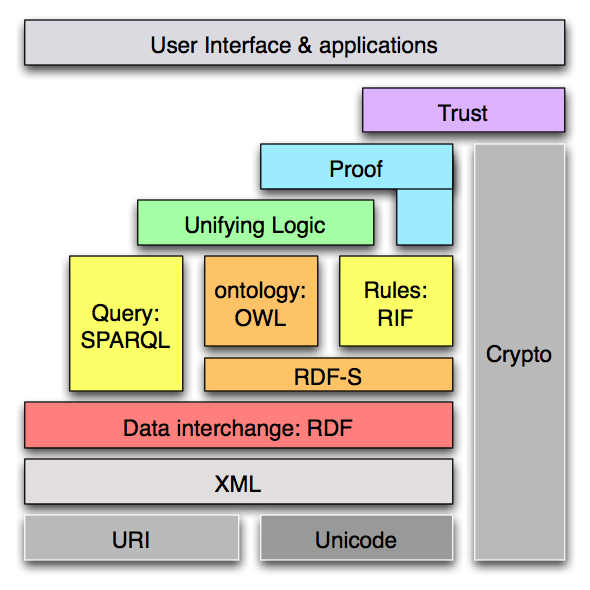
\includegraphics[width=\textwidth]{images/semantic-web-stack.png}
    \end{column}
    \begin{column}{0.5\textwidth}
      A destacar tres (tecnologías) capas:
      \begin{itemize}
	\item \textbf{RDF} (\textit{Resource Description Framework})
	\item \textbf{OWL} (\textit{Web Ontology Language})
	\item \textbf{SPARQL} (\textit{SPARQL Protocol and RDF query language})
      \end{itemize}
    \end{column}
  \end{columns}
}

\section{El proyecto SWAML}

\subsection{Tecnologías implicadas}
\frame
{
  \frametitle{RDF}

  RDF se basa en un modelo de tripletas del tipo \texttt{(sujeto, predicado, objeto)}. El
  sujeto es un recurso que se identifica con una URI, y se relaciona mediante un 
  predicado binario con el objeto, que puede ser otra URI o un literal.

  \begin{center}
    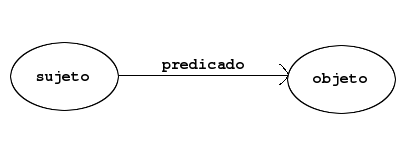
\includegraphics[width=0.6\textwidth]{images/arc.png}
  \end{center}

  Cada tripleta puede verse como un arco, y al juntarse con otros arcos se obtiene
  un grafo dirigido que describe los recursos y las relaciones entre todos los 
  recursos.
}
\frame
{
  \frametitle{SIOC (I)}

  \begin{columns}
   \begin{column}{0.6\textwidth}
     \begin{center}
	\textbf{SIOC} (Semantically-Interlinked Online Communities) es una ontología desarrollada 
	por el equipo de web semántica de DERI Galway para describir semánticamente 
	distintas comunidades online.
     \end{center}
   \end{column}
   \begin{column}{0.4\textwidth}
	
\includegraphics[width=0.9\textwidth]{images/sioc.png}
   \end{column}
  \end{columns}
}
\frame
{
  \frametitle{SIOC (II)}

  \begin{center}
	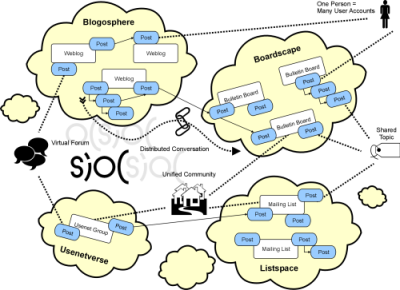
\includegraphics[width=0.85\textwidth]{images/sioc-discussion.png}
  \end{center}
}
\frame
{
  \frametitle{SIOC (III)}

  \begin{center}
	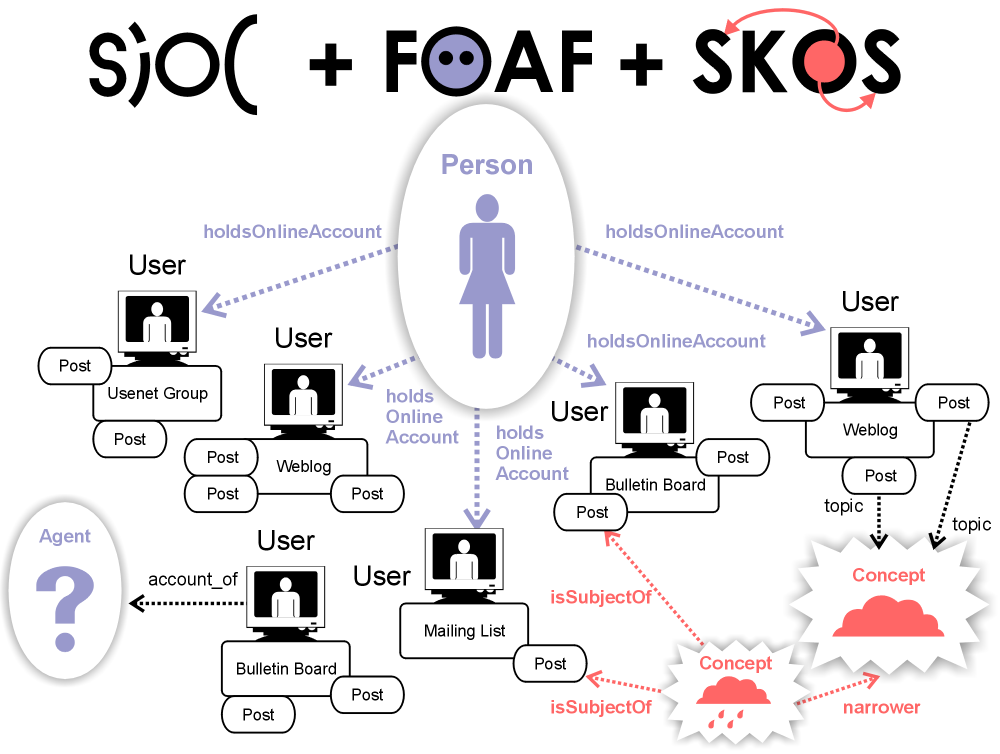
\includegraphics[width=0.8\textwidth]{images/sioc-foaf-skos.png}
  \end{center}
}
\frame
{
  \frametitle{Python}

  \begin{columns}
   \begin{column}{0.6\textwidth}
      \begin{itemize}
	 \item lenguaje de script moderno
	 \item interpretado con tipado dinámico
	 \item orientado a objetos
	 \item multiplataforma
	 \item extensa bliblioteca estandar
	 \item productivo
	 \item maduro
	 \item libre
      \end{itemize}
   \end{column}
   \begin{column}{0.4\textwidth}
	
\includegraphics[width=0.95\textwidth]{images/python.png}
   \end{column}
  \end{columns}
}
\frame
{
  \frametitle{RDFLib}

  RDF se trata de una biblioteca de Python para trabajar con RDF con varias caracteristicas interesantes:

  \begin{itemize}
   \item RDF/XML parser
   \item serialización NTriples, N3 y RDF/XML
   \item soporte para persistencia de grafos en memoria
   \item consultas SPARQL
   \item persistencia
  \end{itemize}

}

\subsection{SWAML}
\frame
{
  \frametitle{SWAML}

  En realidad en proyecto SWAML se compone de varios componentes:

  \begin{itemize}
   \item SWAML propiamente dicho
   \item Buxon
   \item herramientas complementarias
  \end{itemize}
}
\frame
{
  \frametitle{SWAML Core}
  \begin{columns}
   \begin{column}{0.5\textwidth}
	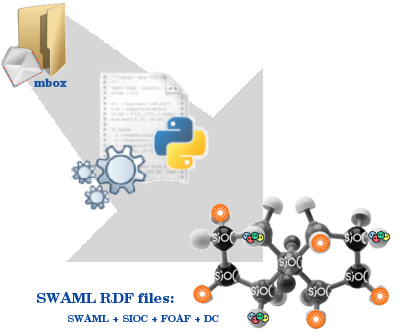
\includegraphics[width=0.95\textwidth]{images/swaml.png}
   \end{column}
   \begin{column}{0.5\textwidth}
	Un proceso batch que se encarga de traducir un mbox a su representación en RDF:
	\begin{enumerate}
	 \item Parsear el mbox
	 \item Recomponer y verificar la consistencia de todos los datos y relaciones
	 \item Serializar a RDF/XML la lista de correo (\texttt{sioc:Forum})
	\end{enumerate}
   \end{column}
  \end{columns}
}
\frame
{
  \frametitle{Buxon}

  Visor de \texttt{sioc:Forum}'s, desarrollado para demostrar que la representación en RDF de una lista de correo
  permite volver recomponerla sin pérdida de información.

  \begin{center}
	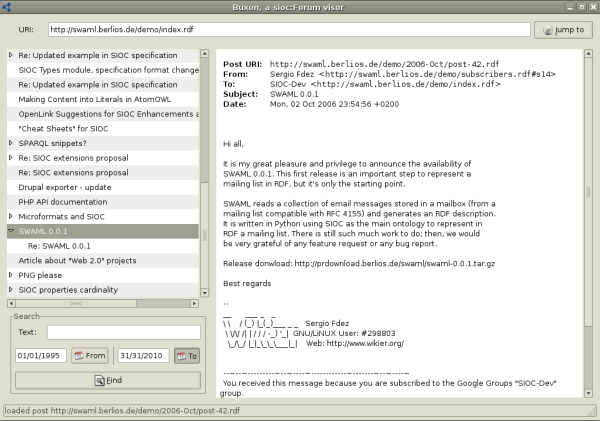
\includegraphics[width=0.7\textwidth]{images/buxon.png}
  \end{center}
}
\frame
{
  \frametitle{Herramientas complementarias}

  Además son necesarias una serie de herramientas adicionales para realizar determinadas tareas:

  \begin{itemize}
   \item \textbf{configWizard}, asistente para realizar configuraciones.
   \item \textbf{FOAF Enricher}, agente encargado de enriquecer la listas de correo con datos sacados de los FOAF de los suscriptores.
   \item \textbf{KML Exporter}, componente encargado de exportar a KML la información geográfica de los suscriptores.
  \end{itemize}
}

\section{Conclusiones}
\subsection{Resultados}
\frame
{
  FIXME\\
  aportación a SIOC
}
\subsection{Futuras líneas de trabajo}
\frame
{
  \frametitle{Futuro inmediato}

  \note[item]{ Usar GMail como fuente de información. }
  \note[item]{ Bastará disponer de una (o varias) cuentas de GMail suscritas a diferentes
    listas de correo. Después apenas habrá que optimizar el software para
    hacer más eficientes estas exportaciones automáticas. }
  \note[item]{ Esperamos llevar a cabo el experimento en la sproximas semanas. }

  \bigskip
  \begin{columns}
   \begin{column}{0.7\textwidth}
    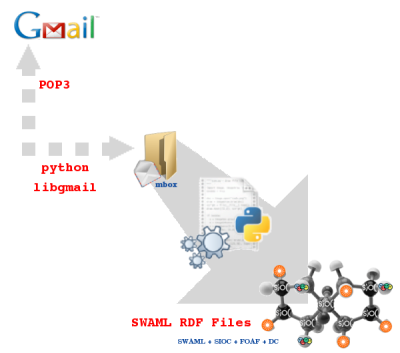
\includegraphics[width=0.99\textwidth]{images/gmail-swaml.png}
   \end{column}
   \begin{column}{0.4\textwidth}
    Automatizar el experimento aislado ya realizado por John Breslin:
    \begin{enumerate}
     \item Descargar los correos (\texttt{python-libgmail})
     \item Generar un mbox
     \item Usar SWAML para generar su descripción en RDF
    \end{enumerate}
   \end{column}
  \end{columns}
  \bigskip
}
\frame
{
  \frametitle{Futuro a medio plazo}
  \begin{itemize}
   \item Marcado semántico para el cuerpo de los mensajes
   \item API en Python para SIOC
   \item Integración con Mailman
   \item API para DIG
  \end{itemize}
}

\section{Demostración}
\subsection{Demostración}
\frame
{
  \note[item]{Crear una configuración en directo con asistente.}
  \note[item]{Ejemplo de exportación con SWAML (con todas las opciones), enseñar los RDF en plano.}
  \note[item]{Mismo ejemplo si enriquecer con FOAF ni exportación a KML.}
  \note[item]{Enriquecer con FOAF.}
  \note[item]{Exportar a KML.}
  \note[item]{Visualizarla con Buxon.}

  \begin{center}
    \LARGE{\textbf{demostración práctica}}
  \end{center}
}
\subsection{Preguntas}
\frame
{
  \note[item]{Agradecer la atención prestada.}
  \note[item]{Quedar a disposición del tribunal para contestar a las
		preguntas o ampliar cualquiera de los temas expuestos.}

  \begin{center}
    \LARGE{\textbf{¿preguntas?}}\\
    \vspace{3cm}
    \small{%
	Esta presentación se distribuye bajo los términos de la licencia
	CreativeCommons Reconocimiento-CompartirIgual 2.5
    }
  \end{center}
}

\appendix

\section{Respuestas preparadas}
\frame{
  FIXME: retocarlas según el tribunal
}


\end{document}
